\documentclass[11pt, a4paper]{article}
\usepackage[spanish]{babel}
\usepackage[utf8]{inputenc}
\usepackage{amsmath, amsfonts}
\usepackage{graphicx}

\begin{document}
\centering
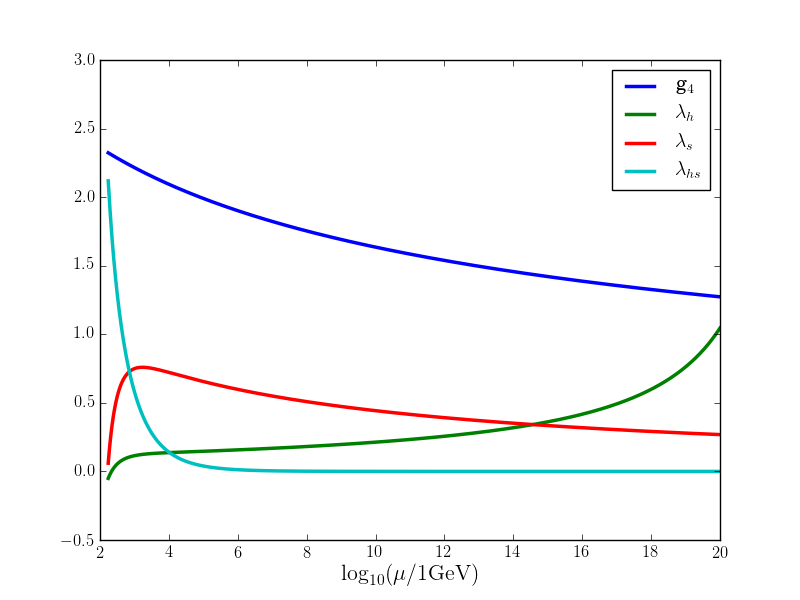
\includegraphics[width=0.7\textwidth]{running}
\begin{itemize}
\item He tenido algunas dificultades al intentar resolver las ecuaciones con \textit{Mathematica}, así que finalmente lo he hecho con \textit{Python}, integrando con el método de Runge-Kutta.
\item En las ecuaciones aparece el Yukawa $y_t$, cuyo \textit{running} depende de las constantes de acoplo de los tres grupos gauge $g_1$, $g_2$, $g_3$. En el artículo desprecian los términos con $g_1$ y $g_2$, yo no lo he hecho (aunque el resultado es similar).
\item Las ecuaciones para $g_1$, $g_2$, $g_3$ y $g_4$ se pueden resolver fácilmente de forma analítica, así que he empleado las soluciones exactas.
\item Para $g_4$ en el artículo no da ningún valor $g_4(\mu_0)$ para fijar la constante de integración.
\item Usando la fórmula (11) del artículo con $N_s=10$ y $N_f=54$, como indican, $g_4$ decrece más rápido que en su gráfica.
\item Modificando el valor de $g_4(m_s)$ las curvas de $\lambda_s$ y $\lambda_{hs}$ apenas cambian. En cambio, la parte de alta energía de $\lambda_h$ es muy sensible a este valor. 
\item Para los valores iniciales de las constantes del potencial he usado $\lambda_s(m_s) = 0$ (como dicen en el pie de la gráfica) y $N_s \lambda_{hs}^2(m_s) = 40$ (la condición para que el Higgs tenga la masa medida, como indican justo antes de la ecuación (12)). 
\item En el caso de $\lambda_h$ tengo más dudas: en la gráfica he usado $\lambda_h=-1/16$. En el artículo dicen que $\hat{\lambda}_h = (\lambda_h + \delta \lambda)e^{4\Gamma}=-1/16$.  Pero haciendo numéricamente la integral para $\Gamma(\mu)$ y sustituyendo para que $\hat{\lambda}_h = -1/16$, se obtiene un valor de $\lambda_h$ mucho menor que el que aparece en la gráfica del artículo. 
\end{itemize}
\end{document}